\apendice{Manual de especificación de diseño}

\section{Diseño arquitectónico}
\subsection{Colocación de los elementos hardware}
La figura \ref{fig:esquemahardware} es un esquema de los componentes hardware y su colocación propuesta en el prototipo, dentro de una riñonera en la cual se sitúan los componentes en 2 capas y una tobillera. Las conexiones entre distintos componentes hardware se representan de forma simplificada mediante flechas moradas. 

Las plataformas sin etiquetar sobre las que están conectados los pulsadores ON/OFF y el sensor MPU-6050 representan dos mitadas de una miniboard (miniplaca de pruebas), la cual se utiliza para conectar estos componentes de forma reversible, permitiendo la corrección de errores o el rediseño del circuito.
\begin{figure}[h]
    \centering
    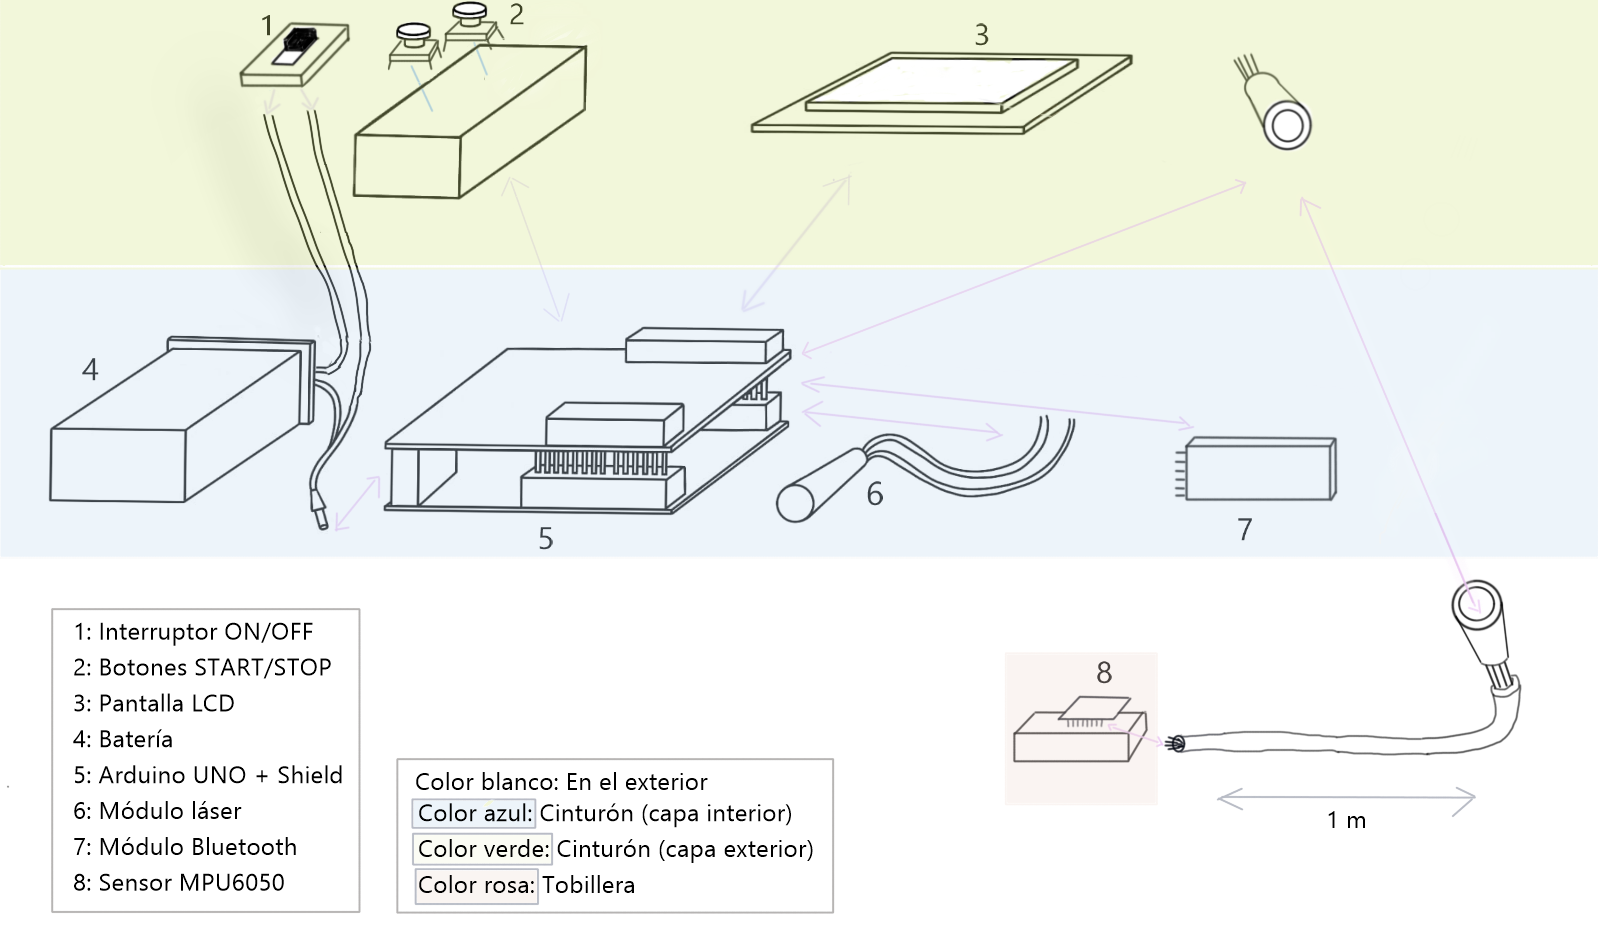
\includegraphics[width=1\textwidth]{img/esquemahardware.png}
    \caption{Esquema del diseño del hardware. Fuente propia}
    \label{fig:esquemahardware}
\end{figure}
\subsection{Conexiones de elementos hardware}
El esquema \ref{fig:circuito} refleja las conexiones requeridas en el circuito que une la placa Arduino UNO con los diferentes módulos y componentes hardware. Es importante recalcar que varios pines de la placa son la fuente de múltiples conexiones, por lo cual se utilizó un Arduino Proto Shield conectado a la placa con el objetivo de aumentar los puntos de conexión a dichos pines mediante soldaduras.
\begin{sidewaysfigure}[h]
    \centering
    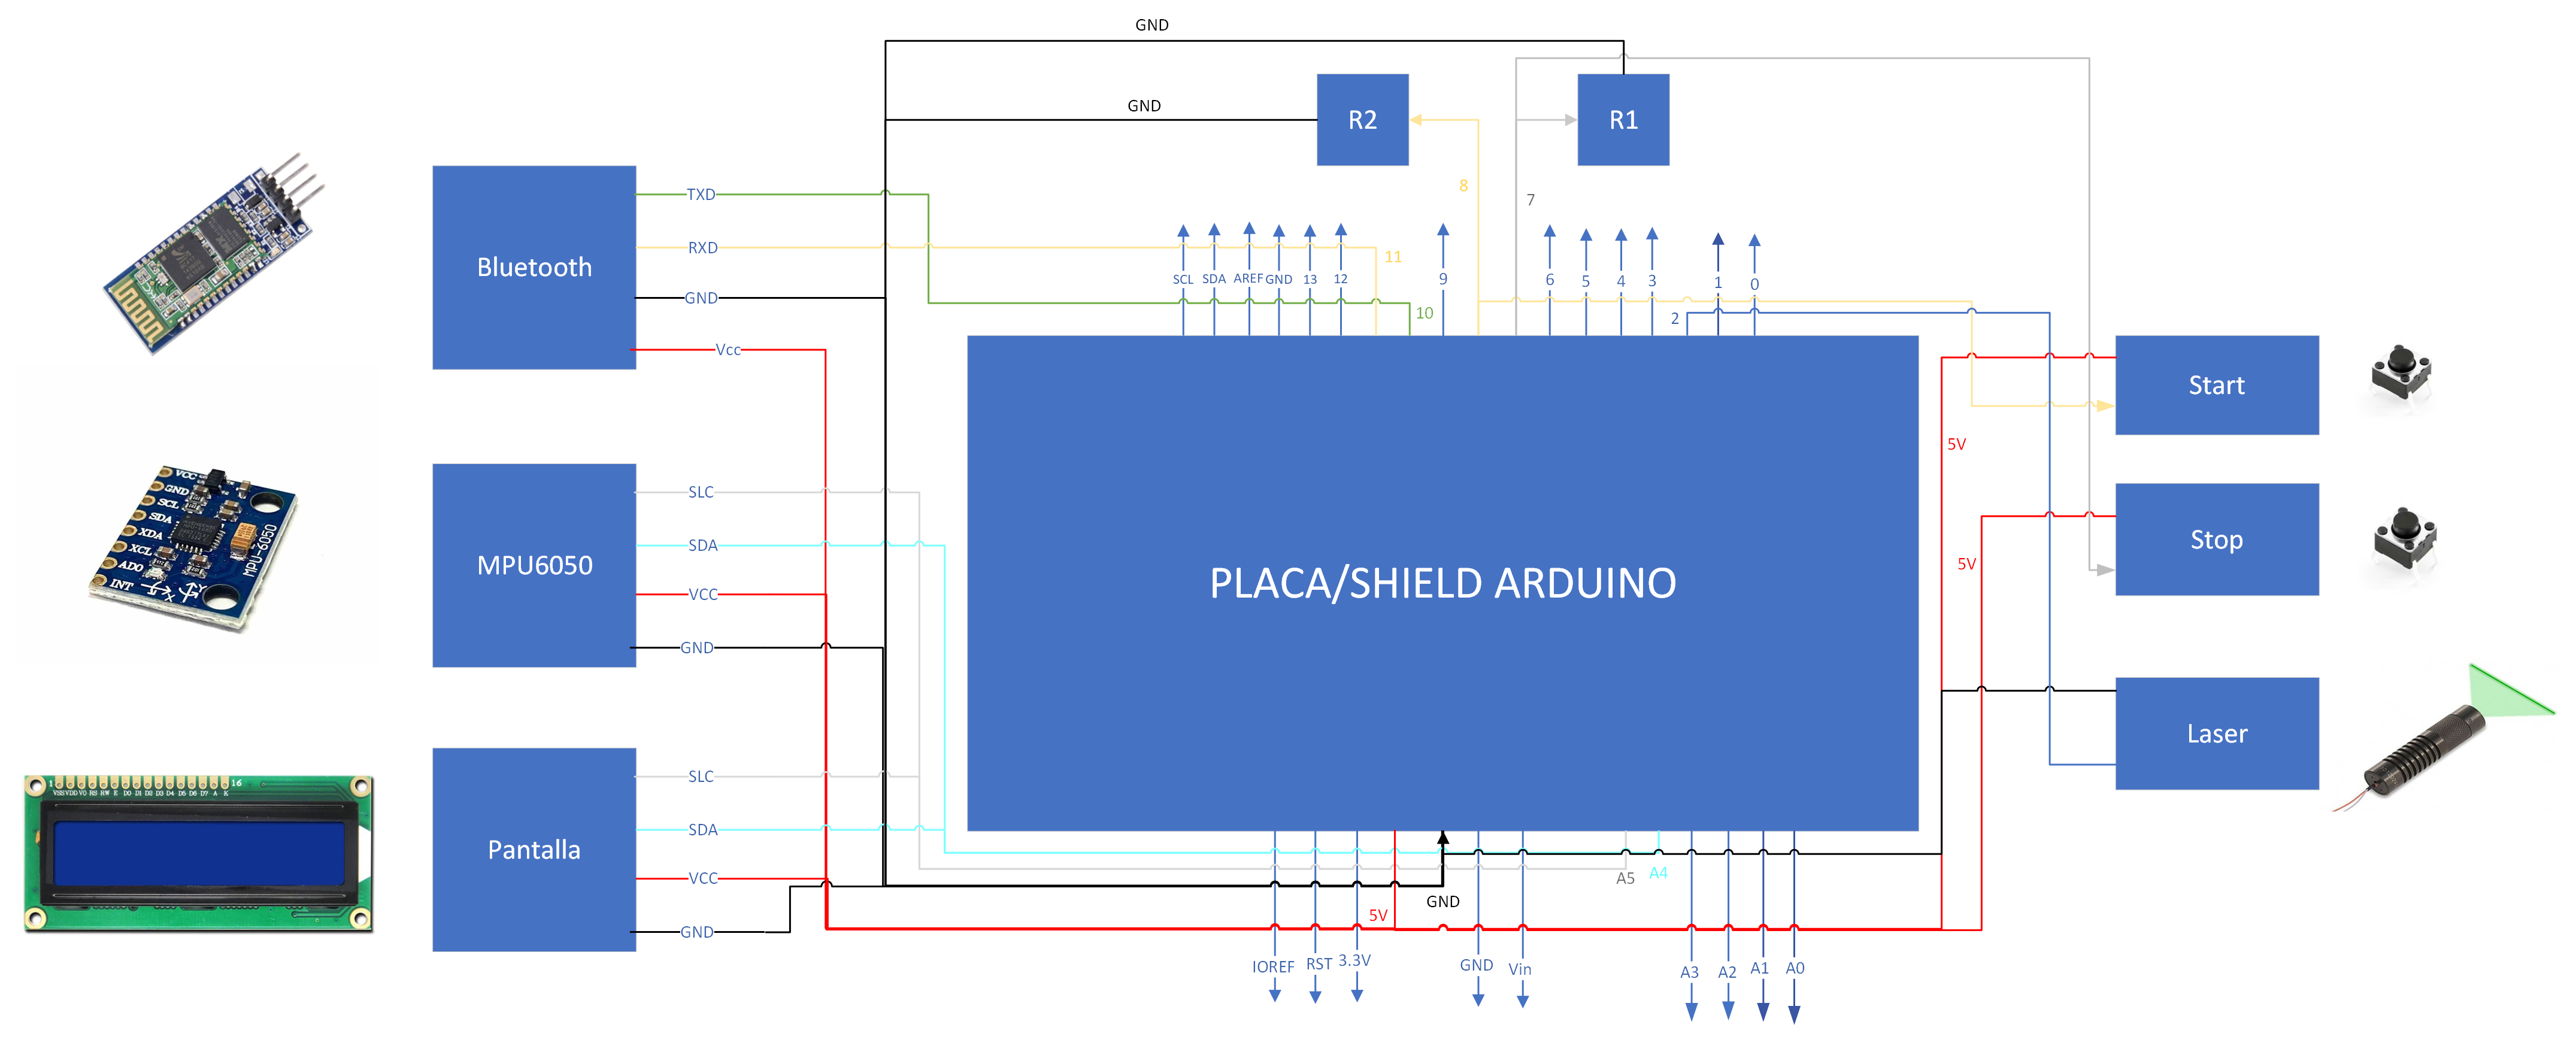
\includegraphics[width=1\textwidth]{img/circuito.png}
    \caption{Esquema de las conexiones de elementos hardware a la placa Arduino UNO. Fuente propia}
    \label{fig:circuito}
\end{sidewaysfigure}

Las conexiones más complicadas son detalladas en las figuras \ref{fig:conexionmpu} (conexión del sensor MPU-6050) \ref{fig:conexionpantalla} (conexión de la pantalla LCD) \ref{fig:conexionpulsadores} (conexión de los pulsadores ON/OFF). Es importante tener en cuenta que estas imágenes son tan sólo una simplificación de las conexiones, ya que tanto los cables como las resistencias que parten de la placa Arduino están soldados en realidad al Proto Shield de Arduino. Adicionalmente, la conexión entre la placa y el sensor MPU-6050 se realiza mediante un cable multihilo, conectado en un extremo a 4 cables provenientes de la placa mediante un conector y en el otro extremo a la mitad de la miniplaca de pruebas donde se conecta el sensor.
\begin{figure}[h]
    \centering
    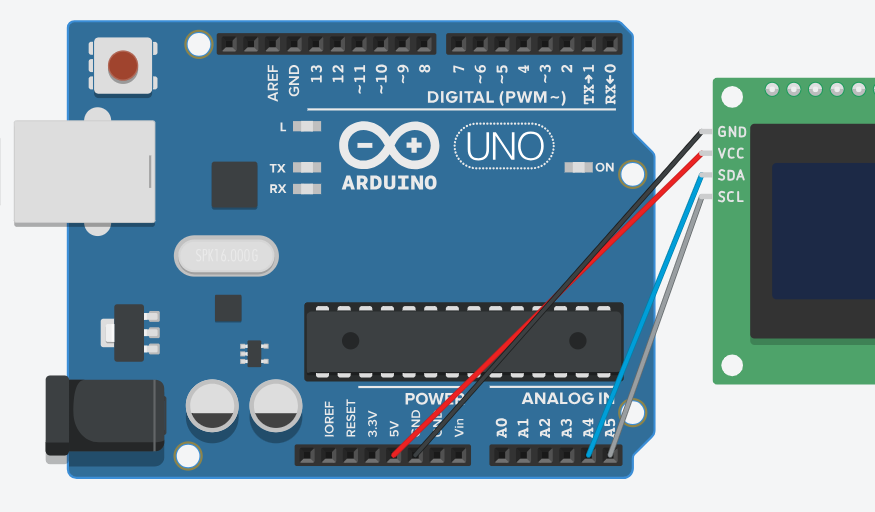
\includegraphics[width=1\textwidth]{img/conexionpantalla.png}
    \caption{Esquema de las conexiones entre la pantalla LCD la placa Arduino UNO mediante el protocolo I2C. Fuente propia}
    \label{fig:conexionpantalla}
\end{figure}
\begin{figure}[h]
    \centering
    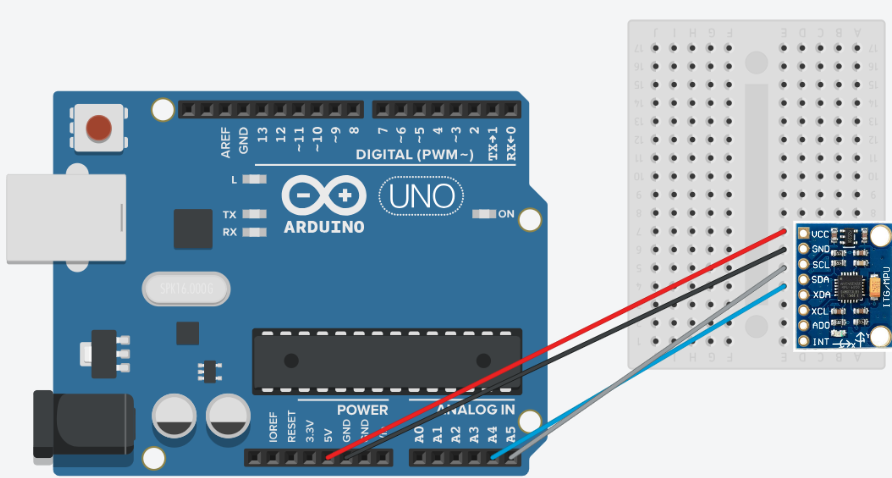
\includegraphics[width=1\textwidth]{img/Conexionmpu.png}
    \caption{Esquema de las conexiones entre el sensor MPU-6050 y la placa Arduino UNO. Fuente propia}
    \label{fig:conexionmpu}
\end{figure}
\begin{figure}[h]
    \centering
    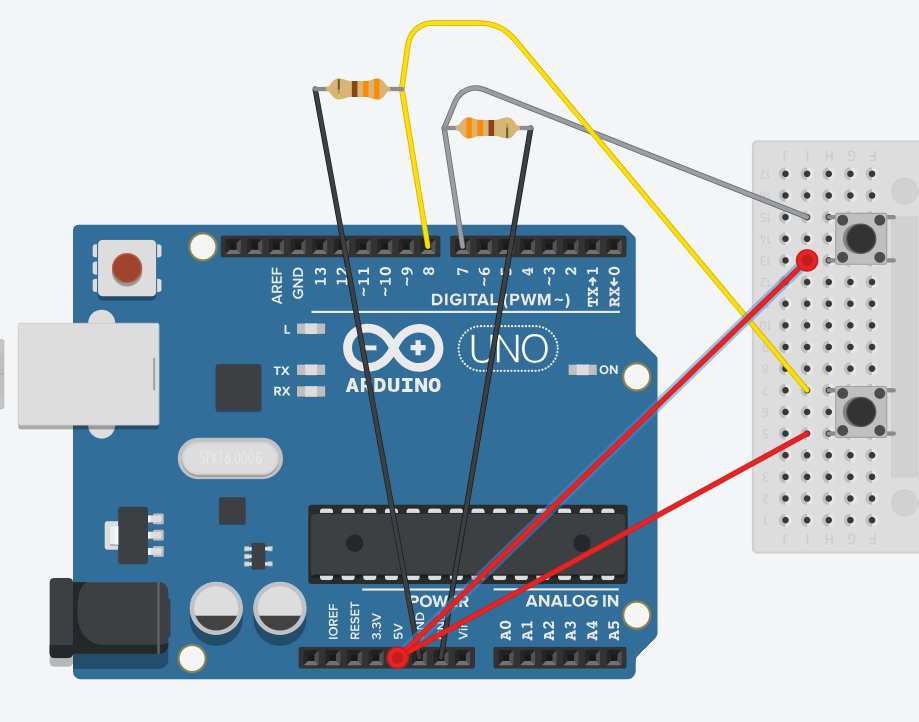
\includegraphics[width=1\textwidth]{img/conexionpulsadores.png}
    \caption{Esquema de las conexiones de los pulsadores ON/OFF a la placa Arduino UNO. Fuente propia}
    \label{fig:conexionpulsadores}
\end{figure}
\subsection{Diagrama de despliegue}
El diagrama de despliegue mostrado en la figura \ref{fig:diagramadespliegue} muestra la estructura y conexiones de los elementos hardware y software que forman el prototipo presentado. Los usuarios acceden mediante su navegador web a la aplicación web, desde la cual hacen uso de diferentes funciones, algunas de las cuales implican el almacenamiento de datos en las tablas de la base de datos 'webparkinson'. Por otro lado, el dispositivo hardware se comunica con el servidor web de la aplicación para enviar datos recogidos por el sensor en tiemo real, recibiendo también información de dicho servidor como comandos.
\begin{figure}[h]
    \centering
    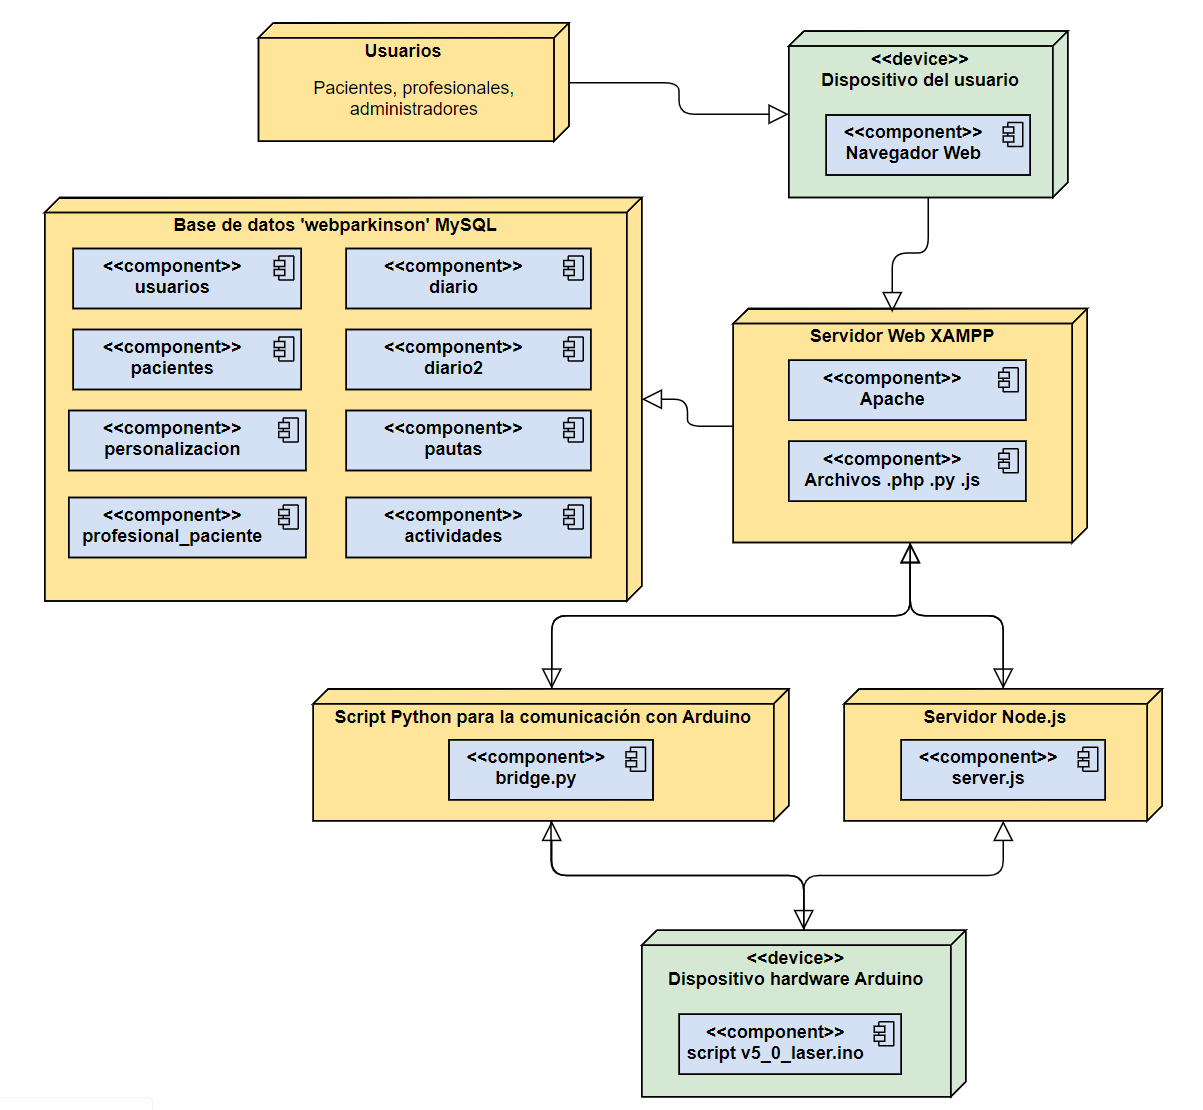
\includegraphics[width=1\textwidth]{img/diagramadespliegue.png}
    \caption{Diagrama de despliegue del sistema. Fuente propia}
    \label{fig:diagramadespliegue}
\end{figure}


